\chapter{Resultados y Discusiones}
El siguiente capitulo se trabajó a base de la forma de validación detallada en el capítulo anterior. Y se detallan los resultados obtenidos.

\section{Detalles de resultados}
Se realizaron varias reuniones con profesores de la materia de Fundamentos de Programación, en estas se revisaron los \textit{puzzles} del juego, se les mostró las mecánicas del juego y se revisó con ellos la forma de instalación. Esto último, dado que por falta de tiempo la instalación se hace por el docente en su propia máquina. Las reuniones se realizaron para ver las opiniones del producto realizado para usuarios finales potenciales. Los usuarios a los que tiene más potencial de afectar el juego son a los estudiantes, pero como los profesores son los que implementan el juego en su clase, es importante de primera mano un estudio para explorar sus perspectivas respecto al juego creado.

Se realizaron reuniones con cinco distintos docentes del departamento de ingeniería eléctrica y computación de la Universidad Autónoma de Ciudad Juárez que imparten o impartieron en los últimos semestres la materia de Fundamentos de Programación en el campus de Ciudad Universitaria.

\subsection{Primera reunión}
Se realizó esta reunión el 6 de octubre del 2021. Se revisó en esta el material del juego, se vio el valor didáctico de los diferentes puzzles del juego y de manera menos detallada, la instalación y el \textit{gameplay}. En esta revisión del juego comento de manera positiva la variedad de los puzzles. Sin embargo, mencionó que debido al diseño de los puzzles que algunos tienen código similar a \textit{C} (figura~\ref{fig:for_puzzle_fail_c}), otro muy parecido a \textit{Python} (figura~\ref{fig:for_puzzle_fail_python}) y algunos adicionales de pseudocódigo, seria complicado para el docente usar este juego para la impartición de su clase porque ``rompería'' con lo visto en clase en algunos temas. Si el profesor tiene que explicar al estudiante que ciertos \textit{puzzles} funcionan de manera diferente a como se explicó en clase, el juego pierda valor didáctico y en el peor de los casos, podría confundir a los estudiantes.
\begin{figure}
    \centering
    \begin{subfigure}{0.4\textwidth}
         \centering
         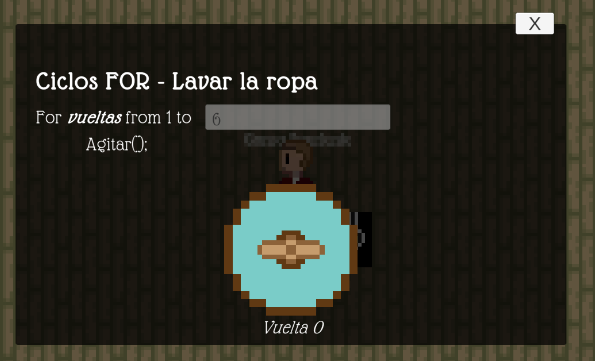
\includegraphics[width=\textwidth]{for_puzzle_fail_python}
         \caption{Este \textit{puzzle} tenía una sintaxis inspirada en \textit{Python} y su uso de \textit{ranges}}
         \label{fig:for_puzzle_fail_python}
     \end{subfigure}
         \begin{subfigure}{0.4\textwidth}
         \centering
         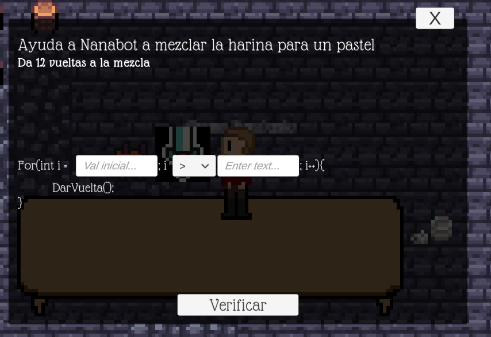
\includegraphics[width=\textwidth]{for_puzzle_fail_c}
         \caption{La sintaxis de este \textit{puzzle} era similar a C}
         \label{fig:for_puzzle_fail_c}
     \end{subfigure}
\end{figure}

Ante estos resultados se decidió volver a analizar el diseño y corregir los detalles encontrados en el producto para que sea posible su uso en el salón de clases. Se cambiaron los ejercicios pertinentes para usar estructuras como lo mencionan el libro \textquotedblleft Fundamentos de programación, algoritmos, estructura de datos y objetos\textquotedblright de Luis Joyanes Aguilar, que está en la carta descriptiva de la materia. Adicionalmente, se resolvió estandarizar todos los ejercicios para que usaran la sintaxis de PSeInt. 

\subsection{Segunda reunión}
Se realizó una reunión el 1 de noviembre del 2021 con otro docente. A partir de esta reunión se usaron los ejercicios rediseñados. Se le mostró los diferentes ejercicios que pueden hacer los jugadores y las mecánicas del juego.

Comento que le pareció muy bien los \textit{puzzles}. Mencionó que los ejercicios de los ciclos y valores booleanos eran muy útiles, destacando que los ejercicios de ciclos donde el jugador tiene que decir cuantas vueltas dan, atacan un problema que ha tenido en sus clases. Adicionalmente detalló que los ejercicios de ciclos que requieren que los jugadores pongan los parámetros correctos son muy útiles porque algunos de sus estudiantes tienen problemas razonando cuando debería terminar el ciclo. Le pareció bien que los ejercicios cambiaran de valores de manera aleatoria, de manera que sea distinta cada partida del juego. 

Agregando a lo anterior, comento positivamente de las mecánicas del juego. Menciono que la forma en la que está el juego puede llamar la atención a los alumnos y mantenerlos interesados en jugar más.

Lo único negativo que menciono es que le gustaría que hubiera ejercicios de arreglos y matrices.

\subsection{Tercera reunión}
El 1 de noviembre del 2021 se tuvo una tercera reunión con otro docente, este no imparte esta clase actualmente, pero lo hizo en semestres anteriores. De la misma manera se le mostró los diferentes ejercicios que resolverán los jugadores y las mecánicas del juego.

Hizo en la reunión las siguientes observaciones de los ejercicios:
\begin{itemize}
    \item Le gustaría que hubiera más ejercicios sobre condicionales dobles.
    \item Comentó que sería bueno agregar títulos en los \textit{puzzle} denotando el tema que trata.
    \item Le gustaría que se agregaran acertijos adicionales que agreguen \textbf{ciclos para} con pasos distintos a 1. Para sacar a los estudiantes fuera de su zona de confort y tendrían la ventaja adicional de crear un modelo mental más robusto.
    \item Las indicaciones de los acertijos deben de ser más claras con lo que se pide.
    \item Quitar las funciones, porque es algo que no se cubre del todo en su clase y los estudiantes se pueden confundir.
    \item Hay algunos lugares (como en el caso de las emergencias) que hay ejercicios no necesariamente de programación. Considera que sería mejor si estos pudieran ser también de programación. Un trabajo a futuro a considerar respecto al juego es un modo de solo programación, donde se quiten preguntas y acertijos que no tengan nada relacionado a la presentación.
\end{itemize}

Adicionalmente, detallo que los estudiantes batallan con las condicionales y los ciclos, este juego tiene el potencial de ayudarles a reforzar su aprendizaje y ayudarles a entender mejor estos temas. Menciono que se le hace interesante este tipo de juego, y cree que los estudiantes les gustara usarlo. Agregando, menciono que le gusto la ambientación del juego.

\subsection{Cuarta reunión}
Se agendó una reunión con un cuarto docente el 3 de noviembre del 2021. 

Este docente consideró que el juego es útil para reforzar lo aprendido en la clase de Fundamentos de Programación, cumpliendo los temas de la materia. Le pareció muy bien que los ejercicios cambiaran cada partida. Además, menciono que le gusto que los puzzles dieran al razonamiento de que hacen los pseudocódigos del ejercicio a resolver; y que en lugar de darles instrucciones y que tengan que escribir un resultado, se les dé un resultado y tengan que evaluar si hace lo que pide las instrucciones.

Lo único que no le convenció del todo fueron la inclusión de funciones en algunos \textit{puzzles}, porque no las ve en su clase y en general es un aspecto nebuloso en la descripción de la materia. Además, lo que le gustaría a futuro es que existiese una versión en un \textit{host}, de manera que puedan mandar a los estudiantes a una \textit{URL} y puedan acceder de esa manera el juego.

Comento que sí usaría este juego, como repaso al final del semestre o para un examen, por la cantidad de temas que trabaja el juego.

\subsection{Quinta reunión}
Se hizo una reunión con un quinto docente el 3 de noviembre del 2021.

Comento que les gustaría más escalones de dificultad, donde los estudiantes tengan que resolver ejercicios más complejos. Y en los puzzles con \textbf{Ciclos Para} agregar ejercicios con pasos negativos y variación de los pasos.

\section{Discusión de los resultados}
A los docentes entrevistados se les hizo interesante el juego, y comentaron que el juego como esta les llamara la atención a sus alumnos cuando lo jueguen.

Sobre los \textit{puzzles}, comentaron positivamente de la variedad que hay. Después de la primera entrevista se notaron puntos débiles que limitarían la adopción del juego en el salón, esto se pudo arreglar, como se había discutido en el capítulo anterior, se cambio a la sintaxis de PSeInt para los puzzles y se ajustaron varios de estos ejercicios para aumentar su valor didáctico. Después de estos cambios, en las reuniones les parecieron bien los ejercicios. Aunque si salieron detalles a corregir, como en algunos ejercicios el tipo de letra hace que los signos sean muy pequeños, hacer las instrucciones más claras y quitar algunas cosas en los pseudocódigos que pudiera agregar ruido a los alumnos.

La opinión general de los docentes inspira confianza a que es algo que usarían o por lo menos algo que considerarían usar una vez desplegado en un servidor.

Salieron algunas sugerencias adicionales, que se discutiran más adelante, son muy interesantes de explorar a futuro y agregarían valor al juego, pero no se pudieron trabajar por falta de tiempo.
